\documentclass{sintefbeamer}

% packages, font, color, and newcommands
\usepackage{amsfonts, amsmath, oldgerm, lmodern}
\usepackage{xeCJK}
\usefonttheme{serif}

% meta-data
\title{深圳大学 Beamer 模板主题}
\subtitle{使用 \LaTeX\ 制作演示文稿}
\author{\href{sota@connect.polyu.hk}{IP 属地中国}}
\date{制作于 2022 年 5 月 22 日}
\titlebackground{images/background}

% document body
\begin{document}

\maketitle

\begin{frame}

本模版基于 \hrefcol{mailto:federico.zenith@sintef.no}{Federico Zenith} 发布的 \hrefcol{https://www.overleaf.com/latex/templates/sintef-presentation/jhbhdffczpnx}{SINTEF Presentation} 模版二次修改制作而成\vspace{\baselineskip}

后文为 \hrefcol{mailto:federico.zenith@sintef.no}{Federico Zenith} 为模版提供的简明教程,版权归其所有\vspace{\baselineskip}

本模版根据 \hrefcol{https://creativecommons.org/licenses/by-nc/4.0/legalcode}{Creative Commons CC BY 4.0} 进行授权

\end{frame}

\section{\LaTeX\ 与 Beamer 简介}

\begin{frame}{Beamer for SINTEF slides}{\thesection \, \secname}

\begin{itemize}
\item We assume you can use \LaTeX; if you cannot,
\hrefcol{http://en.wikibooks.org/wiki/LaTeX/}{you can learn it here}
\item Beamer is one of the most popular and powerful document
classes for presentations in \LaTeX
\item Beamer has also a detailed
\hrefcol{http://www.ctan.org/tex-archive/macros/latex/contrib/beamer/doc/beameruserguide.pdf}{user manual}
\item Here we will present only the most basic features to get you up to speed
\end{itemize}
\end{frame}

\begin{frame}{Beamer vs. PowerPoint}
Compared to PowerPoint, using \LaTeX\ is better because:
\begin{itemize}
\item It is not What-You-See-Is-What-You-Get, but
What-You-\emph{Mean}-Is-What-You-Get:\\
you write the content, the computer does the typesetting
\item Produces a \texttt{pdf}: no problems with fonts, formulas,
      program versions
\item Easier to keep consistent style, fonts, highlighting, etc.
\item Math typesetting in \TeX\ is the best:
\begin{equation*}
\mathrm{i}\,\hslash\frac{\partial}{\partial t} \Psi(\mathbf{r},t) =
-\frac{\hslash^2}{2\,m}\nabla^2\Psi(\mathbf{r},t)
+ V(\mathbf{r})\Psi(\mathbf{r},t)
\end{equation*}

\end{itemize}
\end{frame}

\section{编辑方法}

\begin{frame}[fragile]{Selecting the Class}
After the last update to the graphic profile, the \texttt{sintef} theme for
Beamer has been updated into a full-fledged class.
To start working with \texttt{sintefbeamer}, start a \LaTeX\ document with the
preamble:
\begin{block}{Minimum SINTEF Beamer Document}
\verb|\documentclass{sintefbeamer}|\\
\verb|\begin{document}|\\
\verb|\begin{frame}{Hello, world!}|\\
\verb|\end{frame}|\\
\verb|\end{document}|\\
\end{block}
\end{frame}

\begin{frame}[fragile]{Title page}
To set a typical title page, you call some commands in the preamble:
\begin{block}{The Commands for the Title Page}
\begin{verbatim}
\title{Sample Title}
\subtitle{Sample subtitle}
\author{First Author, Second Author}
\date{Defaults to today's}
\end{verbatim}
\end{block}
You can then write out the title page with \verb|\maketitle|.

You can set a different background image than the default one with the
\verb|\titlebackground| command, set before \verb|\maketitle|.

In the \texttt{backgrounds} folder, you can find a lot of standard backgrounds
for SINTEF presentation title pages.

\end{frame}

\begin{frame}[fragile]{Writing a Simple Slide}
\framesubtitle{It's really easy!}
\begin{itemize}[<+->]
\item A typical slide has bulleted lists
\item These can be uncovered in sequence
\end{itemize}
\begin{block}{Code for a Page with an Itemised List}<+->
\begin{verbatim}
\begin{frame}
  \frametitle{Writing a Simple Slide}
  \framesubtitle{It's really easy!}
  \begin{itemize}[<+->]
    \item A typical slide has bulleted lists
    \item These can be uncovered in sequence
  \end{itemize}
\end{frame}\end{verbatim}
\end{block}
\end{frame}

\begin{frame}[fragile]{Adding images}
\begin{columns}
\begin{column}{0.7\textwidth}
Adding images works like in normal \LaTeX:
\begin{block}{Code for Adding Images}
\begin{verbatim}
\usepackage{graphicx}
% ...
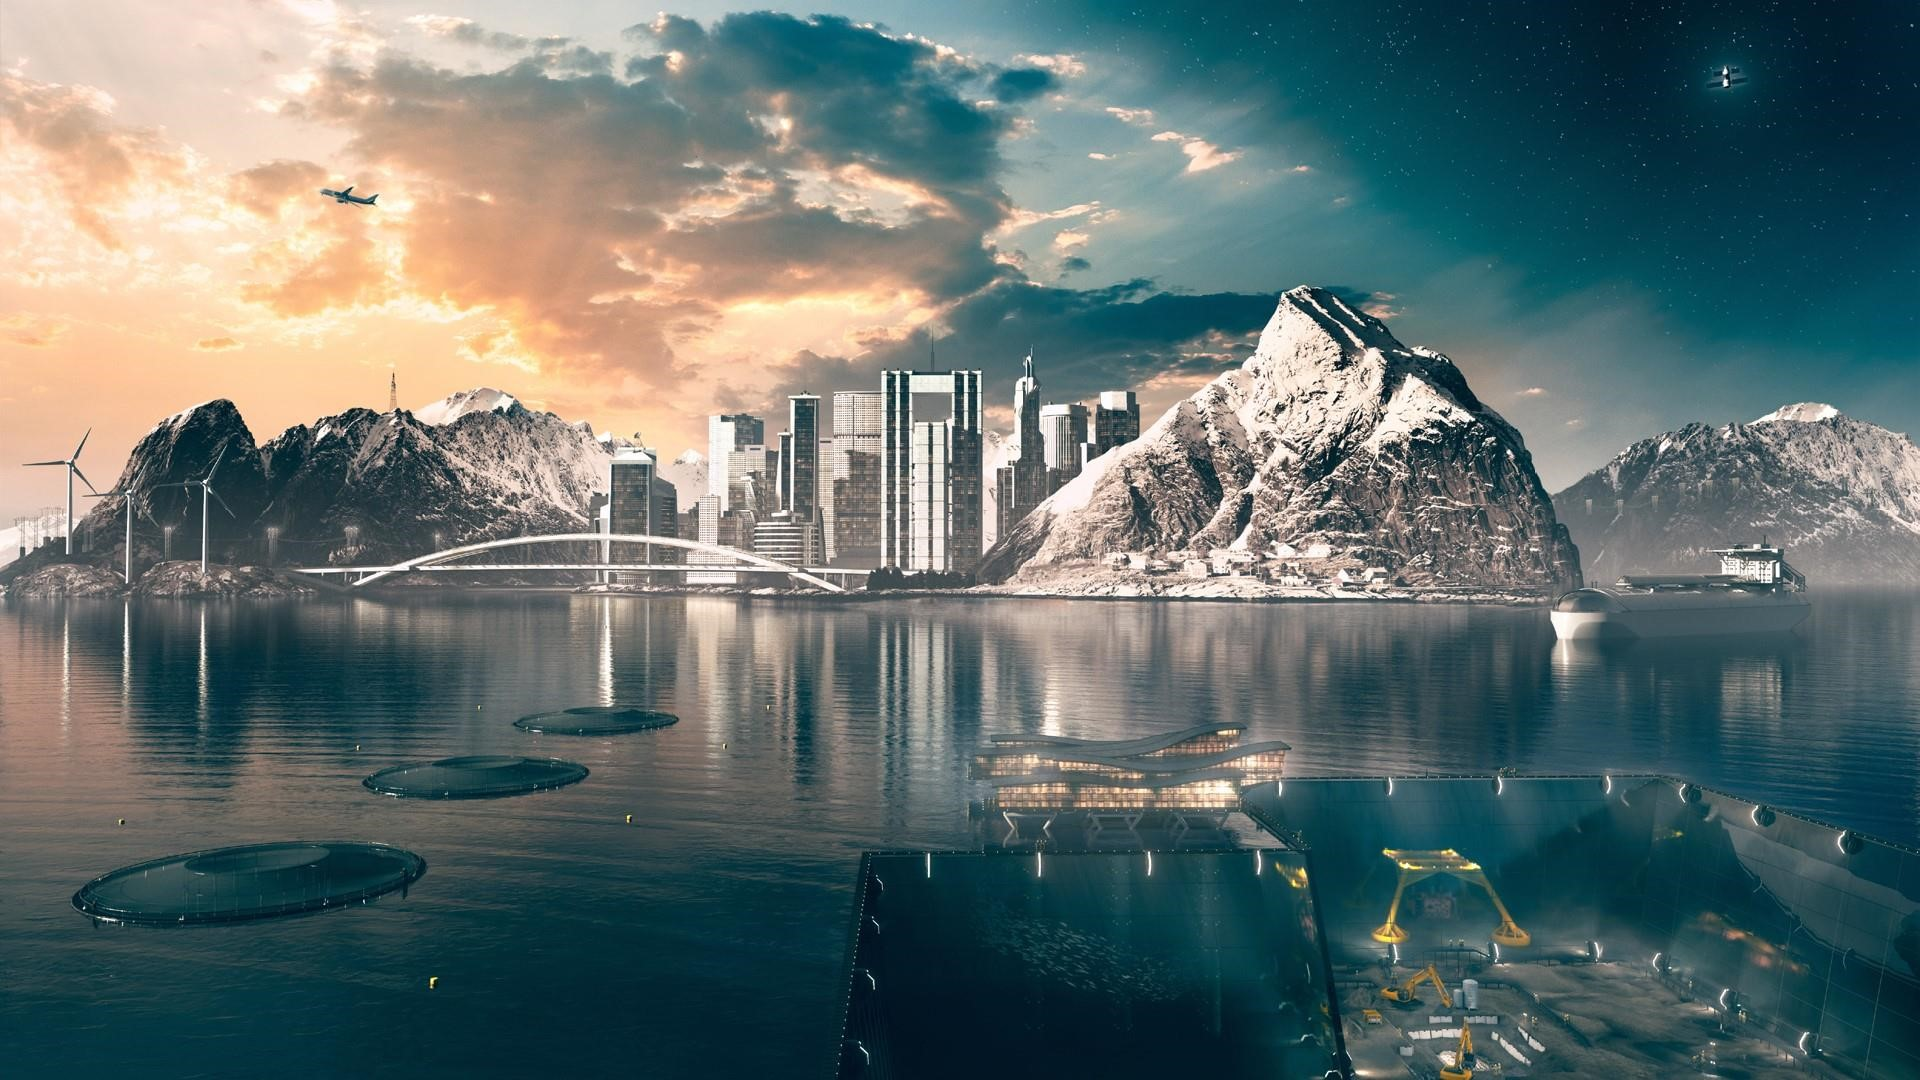
\includegraphics
[width=\textwidth]{images/default}
\end{verbatim}
\end{block}
\end{column}
\begin{column}{0.3\textwidth}
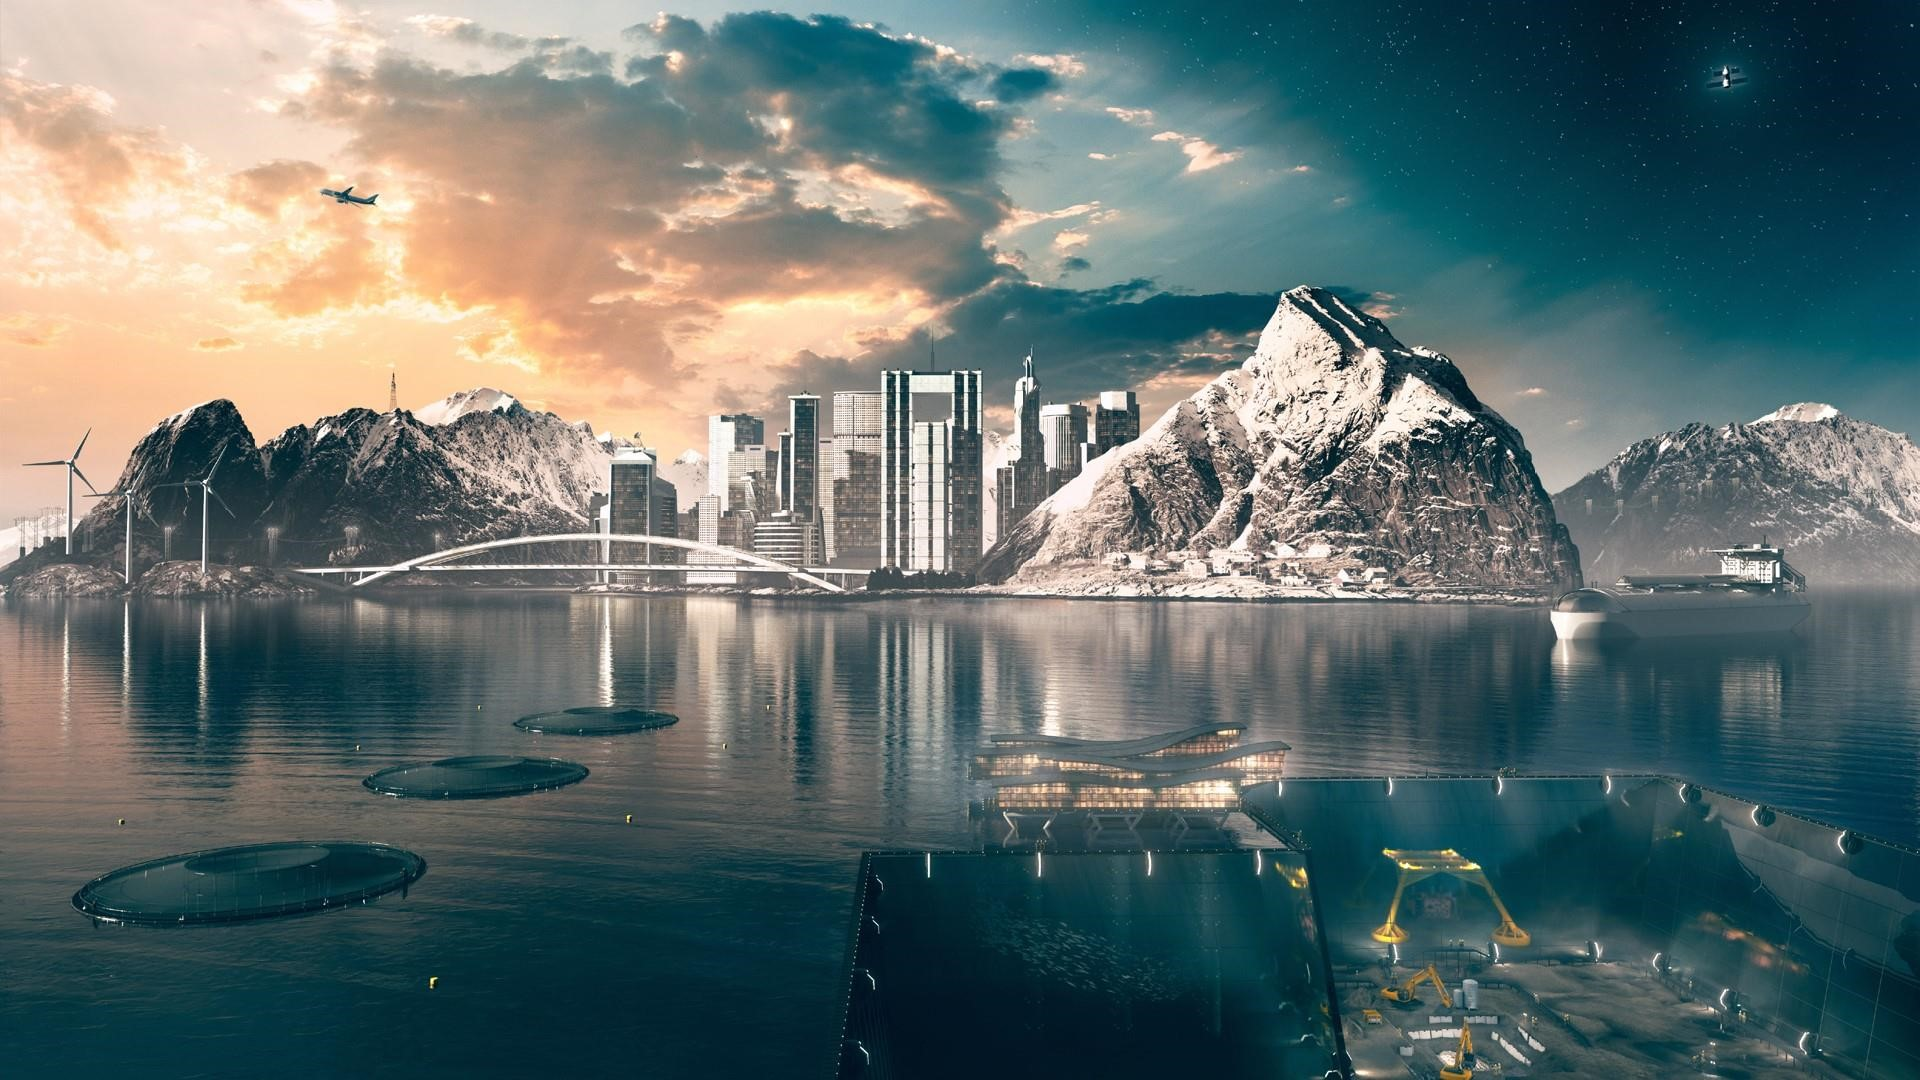
\includegraphics
[width=\textwidth]{images/default}\\
\end{column}
\end{columns}
\end{frame}

\begin{frame}[fragile]{Splitting in Columns}
Splitting the page is easy and common;
typically, one side has a picture and the other text:
\begin{columns}
\begin{column}{0.6\textwidth}
This is the first column
\end{column}
\begin{column}{0.3\textwidth}
And this the second
\end{column}
\end{columns}
\begin{block}{Column Code}
\begin{verbatim}
\begin{columns}
    \begin{column}{0.6\textwidth}
        This is the first column
    \end{column}
    \begin{column}{0.3\textwidth}
        And this the second
    \end{column}
    % There could be more!
\end{columns}
\end{verbatim}
\end{block}
\end{frame}

\begin{frame}[fragile]
\frametitle{Fonts}
\begin{itemize}
\item The paramount task of fonts is being readable
\item There are good ones...
  \begin{itemize}
  \item {\textrm{Use serif fonts only with high-definition projectors}}
  \item {\textsf{Use sans-serif fonts otherwise (or if you simply prefer them)}}
  \end{itemize}
\item ... and not so good ones:
  \begin{itemize}
  \item {\texttt{Never use monospace for normal text}}
  \item {\frakfamily Gothic, calligraphic or weird fonts: should always: be
  avoided}
\end{itemize}
\end{itemize}
\end{frame}

\begin{frame}[fragile]{Look}
\begin{itemize}
\item To change the colour of the title dash, give one of the class options
      \texttt{cyandash} (default), \texttt{greendash}, \texttt{magentadash},
      \texttt{yellowdash}, or \texttt{nodash}.
\item To change between the light and dark themes, give the class options
      \texttt{light} (default) or \texttt{dark}. It is not possible to switch
      theme for one slide because of the design of Beamer---and it's probably a
      good thing.
\item To insert a final slide, use \verb|\backmatter|.
\item The aspect ratio defaults to 16:9, but you can change it to 4:3 for old
      projectors by passing the class option \texttt{aspectratio=43}; any other
      values accepted by Beamer are also possible.
\end{itemize}
\end{frame}

\section{总结}

\begin{frame}
\frametitle{Good Luck!}
\begin{itemize}
\item Enough for an introduction! You should know enough by now
\item If you have corrections or suggestions,
\hrefcol{mailto:federico.zenith@sintef.no}{send them to me!}
\end{itemize}
\end{frame}

\backmatter

\end{document}
